\documentclass[11pt,a4paper,onecolumn]{article}
\usepackage{amssymb,amsmath,amsfonts}
\usepackage{bm}
\usepackage[margin = 1.5cm,
		    marginparsep = 0.2cm,
			headsep = 0.5cm,
			footskip = 0.7cm, 	
			marginparwidth = 1cm]{geometry}
%\usepackage{showframe}			

\usepackage{indentfirst}
\usepackage{calc}
\pagestyle{empty}
\usepackage{physsummer}

\setlength{\parindent}{0pt}
\setlength{\parskip}{0pt}

%% Рисование районного тура с двумя шапками:
%% Следует использовать так:
%% 		\OlympSetReg{ год в формате 16/17 }{ класс }{ номер варианта }{ условие }
\newcommand{\OlympSetRegRussia}[4]{  %% Районный тур всероссийской
	\setcounter{notask}{1}
	\begin{center}
		\textsc{ Всероссийская олимпиада школьников по физике 20#1 г. } \\
		\textsc{ Районный этап } \\
		\textit{ Решения см. на сайте { \underline{www.physolymp.spb.ru} } } \\
	\end{center}
	\vspace{ -1cm }
	\parbox{ 0.5\textwidth }{ \flushleft  \textsc{#2 класс} }
	\parbox{ 0.5\textwidth }{ \flushright \textsc{#3-й вариант } } \\[ 0.1cm ]
	#4
	\vfill
	\begin{center}
		\textsc{Оставьте условие себе!}
	\end{center}
	\clearpage
}

\newcommand{\OlympSetRegSPb}[4]{ 	
	\setcounter{notask}{1}
	\begin{center}
		\textsc{ Городская открытая олимпиада школьников по физике  20#1 г. } \\
		\textsc{ Отборочный этап } \\
		%\textsc{ I городской тур } \\
		\textit{ Решения см. на сайте { \underline{www.physolymp.spb.ru} } } \\
	\end{center}
	\vspace{ -1cm }
	\parbox{ 0.5\textwidth }{ \flushleft  \textsc{#2 класс } }
	\parbox{ 0.5\textwidth }{ \flushright \textsc{#3-й вариант } }\\[ 0.1cm ]
	#4
	\vfill
	\begin{center}
		\textsc{Оставьте условие себе!}
	\end{center}
	\clearpage	
}


%% Рисование городского тура с выводом

\newcommand{\OlympHeader}[4]{
	\setcounter{notask}{1}
	\begin{center}
		\textsc{  Городская открытая олимпиада школьников по физике 20#1 г. } \\
		%\textsc{ Основной этап } \\
		\textsc{ Теоретический тур } \\
		\textit{ Решения см. на сайте { \underline{www.physolymp.spb.ru} } } \\
	\end{center}
	\vspace{ -1cm }
	\parbox{ 0.5\textwidth }{ \flushleft  \textsc{#2 класс} }
	\parbox{ 0.5\textwidth }{ \flushright  \textsc{Первый этап} }
		#3
	\vfill
	\begin{center}
		\textsc{Оставьте условие себе!}
	\end{center}
	\clearpage
	
	\begin{center}
		\textsc{  Городская открытая олимпиада школьников по физике 20#1 г. } \\
		%\textsc{ Основной этап } \\
		\textsc{ Теоретический тур } \\
		\textit{ Решения см. на сайте { \underline{www.physolymp.spb.ru} } } \\
	\end{center}
	\vspace{ -1cm }
	\parbox{ 0.5\textwidth }{ \flushleft  \textsc{8 класс} }
	\parbox{ 0.5\textwidth }{ \flushright  \textsc{Второй этап} }
		#4
	\vfill
	\begin{center}
		\textsc{Оставьте условие себе!}
	\end{center}
	\clearpage	
}


\setcounter{notask}{1}

\usepackage{libertine}
\begin{document}

\OlympSetRegRussia{18/19}{7}{1}
{ 
\taskpic { Автомобиль выехал из пункта $A$ в пункт $D$, по дороге проезжая пункты $B$ и $C$. Расстояние между всеми соседними пунктами $60\unit{км}$. Максимально разрешенная скорость на дороге между пунктами $A$ и $B$ составляет $60\unit{км/ч}$, между $B$ и $C$ --- $90\unit{км/ч}$, между $C$ и $D$ --- $120\unit{км/ч}$. Вдоль дороги поставлены три камеры, которые фиксируют, в какое время мимо нее проезжает автомобиль. Первая камера в пункте $A$, вторая посередине между $B$ и $C$, и третья в пункте $D$. Автомобиль проезжает первую в $13$:$20$, вторую в $14$:$30$ и третью в $15$:$30$. На участках между какими камерами автомобиль точно превысил скоростной режим?}{ \begin{tikzpicture}
	\draw[very thick] (0, 0) -- (3, 0);
	\fill (0, 0)node[above]{$A$} circle (0.1);
	\fill (1, 0)node[above]{$B$} circle (0.1);
	\fill (2, 0)node[above]{$C$} circle (0.1);
	\fill (3, 0)node[above]{$D$} circle (0.1);
	\draw [dashed] (0, 0) -- (0, -1);
	\draw [dashed] (1, 0) -- (1, -1);
	\draw [dashed] (2, 0) -- (2, -1);
	\draw [dashed] (3, 0) -- (3, -1);
	\draw [<->] (0, -1) -- (1, -1)node[midway, below]{\scriptsize{$60\text{~км}$}};
	\draw [<->] (1, -1) -- (2, -1)node[midway, below]{\scriptsize{$60\text{~км}$}};
	\draw [<->] (2, -1) -- (3, -1)node[midway, below]{\scriptsize{$60\text{~км}$}};
	\draw[rounded corners=0.7] (-0.2, 1) rectangle +(0.4, -0.3);
	\draw (-0.05, 0.85) circle (0.1); 
	\draw (0.14, 0.95) ellipse (0.05 and 0.03);
	\draw[rounded corners=0.7] (1.3, 1) rectangle +(0.4, -0.3);
	\draw (1.45, 0.85) circle (0.1); 
	\draw (1.64, 0.95) ellipse (0.05 and 0.03);
	\draw[rounded corners=0.7] (2.8, 1) rectangle +(0.4, -0.3);
	\draw (2.95, 0.85) circle (0.1); 
	\draw (3.14, 0.95) ellipse (0.05 and 0.03);
\end{tikzpicture}}
\task { Завхоз купил в столовую большую бутылку жидкого мыла. Через неделю он обнаружил, что посетители израсходовали все мыло. Тогда завхоз купил такую же новую бутылку, но в целях экономии решил доливать в нее воду доверху каждый раз, когда уровень жидкости опускается до трети. Известно, что каждое разбавление посетители замечают и начинают выдавливать в $3$ раза больше жидкости. Через сколько дней мыло в бутылке закончится?  Каждый день приходит одинаковое число посетителей.}
\taskpic {  Автобус движется по шоссе, вдоль которого на одинаковом расстоянии стоят фонари, а за ними на одинаковом расстоянии посажены деревья. Через щель между занавесками мальчик наблюдает за фонарями и деревьями. Мальчик всегда видит ровно $4$ дерева и $3$ фонаря. Известно также, что от одного конца щели до другого каждое дерево проходит за $3\unit{секунды}$, а фонарь --- за $1\unit{секунду}$. Найдите, сколько деревьев за время пути успел насчитать мальчик, если он насчитал $180$ фонарей. }{ \input{Problems/pic/reg19-07-3-pic.tex}}
\task { В удалении от железнодорожных путей находится пулемёт, который стреляет очередями по $300$ выстрелов в минуту, поворачивая дуло слева направо. Известно, что расстояние между соседними дырками от пуль в поезде, едущем направо, равно $30$ см, а в поезде, едущем налево --- $100$ см. Все поезда ездят с одинаковой постоянной скоростью. Найдите эту скорость.}
\task { В обычном режиме работы станции метро пассажиры спускаются, используя две стороны одного эскалатора. На правой стороне пассажиры стоят, на левой~--- идут пешком. Когда поток пассажиров, входящих на станцию, увеличился, у эскалатора начала скапливаться очередь. Через минуту по громкой связи объявили стоять на эскалаторе с левой и правой стороны, и очередь начала расти быстрее. Еще через минуту люди поняли, что нужно что-то менять, и стали спускаться пешком по обеим сторонам эскалатора, после чего очередь стала сокращаться. На графике представлена зависимость количества человек в очереди от времени. Найдите, через сколько минут очередь у эскалатора сократится до нуля.}
\begin{figure}[h!]
	\centering
	\begin{tikzpicture}[scale=0.92,
	/pgfplots/axis labels at tip/.style={ 
		xlabel style={ at={ (current axis.right of origin) }, 
			yshift = 1 ex,
			anchor = south east,
			fill=white}, 
		ylabel style={ at={ (current axis.above origin) }, 
			xshift = 1 ex, 
			anchor = north west,
			fill = white} } ]
	\begin{axis}[
	grid style={line width=0.1pt, draw=gray!80},
		line width = 2pt, 
		axis x line = middle,
		axis y line = middle,
		axis labels at tip,
		xmin = 0, xmax = 3.5,
		ymin = 0, ymax = 55,
		xtick = {0, 1, ..., 3},
		ytick = {0, 10, ..., 50},
		xlabel = {$t,\text{ мин }$},
		ylabel = {$L,\text{ чел}$},
		grid = both,
		major grid style={line width = 1.3pt,draw=black!50},
		minor grid style={line width=.4pt, draw=black!50},
		major tick length = 7pt,
	    every major tick/.style={
			black,
	        line width = 2pt,
        },
		minor tick length = 4pt,
	    every minor tick/.style={
			black,
	        line width = 1pt,
        },
		minor tick num = 0]
	\draw [line width = 2pt] 
		(0, 0) to (1, 10) to (2, 50);
%	\draw (15,0) to ++ (180, 90);
%	\draw [line width = 2pt]	(0, 0) to (120, 60);
%	\draw (170, 100) node [anchor = south, rectangle, draw, fill = white] {Город};
%	\draw (0,100) to node [midway, above] {Город}(180, 100);
	\end{axis}
	\end{tikzpicture}
\end{figure}
}

\newpage

\OlympSetRegRussia{18/19}{7}{2}
{ 
\taskpic { Автомобиль выехал из пункта $A$ в пункт $D$ по дороге проезжая пункты $B$ и $C$. Расстояние между всеми соседними пунктами $100\unit{км}$. Максимально разрешенная скорость на дороге между пунктами $A$ и $B$ составляет $50\unit{км/ч}$, между $B$ и $C$ --- $75\unit{км/ч}$, между $C$ и $D$ --- $100\unit{км/ч}$. Вдоль дороги поставлены три камеры, которые фиксируют, в какое время мимо нее проезжает автомобиль. Первая камера в пункте $A$, вторая посередине между $B$ и $C$, и третья в пункте $D$. Автомобиль проезжает первую в $16$:$30$, вторую в $19$:$30$ и третью в $21$:$00$.  На участках между какими камерами автомобиль точно превысил скоростной режим?}{ \input{Problems/pic/reg19-07-1-a-pic.tex}}
\task { Завхоз купил в столовую большую бутылку жидкого мыла. Через неделю он обнаружил, что посетители израсходовали все мыло. Тогда завхоз купил такую же новую бутылку, но в целях экономии решил доливать в нее воду доверху каждый раз, когда уровень жидкости опускается до четверти. Известно, что каждое разбавление посетители замечают и начинают выдавливать в $4$ раза больше жидкости. Через сколько дней мыло в бутылке закончится?  Каждый день приходит одинаковое число посетителей.}
\taskpic {  Автобус движется по шоссе, вдоль которого на одинаковом расстоянии стоят фонари, а за ними на одинаковом расстоянии посажены деревья. Через щель между занавесками мальчик наблюдает за фонарями и деревьями. Мальчик всегда видит ровно $2$ дерева и $3$ фонаря. Известно также, что от одного конца щели до другого каждое дерево проходит за $4\unit{секунды}$, а фонарь --- за $1.5\unit{секунды}$. Найдите, сколько фонарей за время пути успел насчитать мальчик, если он насчитал $30$ деревьев. }{ 
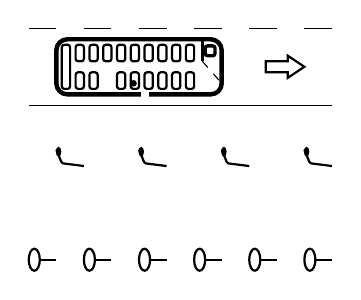
\begin{tikzpicture}[scale = 0.7, rotate = 180]
	\draw (-2, 1.2) -- (3.5, 1.2);
	\draw (-2, -0.2) -- (-1.5, -0.2);
	\draw (-1, -0.2) -- (-0.5, -0.2);
	\draw (0, -0.2) -- (0.5, -0.2);
	\draw (1, -0.2) -- (1.5, -0.2);
	\draw (2, -0.2) -- (2.5, -0.2);
	\draw (3, -0.2) -- (3.5, -0.2);
	\draw[thick] (-1.5, 0.5) -- +(0.3, 0.2) -- +(0.3, 0.1) -- +(0.7, 0.1) -- +(0.7, -0.1) -- +(0.3, -0.1) -- +(0.3, -0.2) -- cycle;
%%%%%%%%%%%	
	\draw[ultra thick, rounded corners] (0, 0) rectangle (3, 1);
	\fill[white] (1.32, 0.96) rectangle +(0.15, 0.1);
	\draw[thick, rounded corners = 0.9] (2.9, 0.1) rectangle +(-0.15, 0.8);
	\draw[very thick, rounded corners = 0.9] (0.12, 0.12) rectangle +(0.18, 0.18);
	\draw[thick] (0.35, 0) -- (0.35, 0.4);
	\draw[dashed] (0.35, 0.4) -- (0, 0.8);	
	\draw[thick, rounded corners = 0.9] (0.5, 0.1) rectangle +(0.15, 0.3);
	\draw[thick, rounded corners = 0.9] (0.5, 0.6) rectangle +(0.15, 0.3);
	\draw[thick, rounded corners = 0.9] (0.75, 0.1) rectangle +(0.15, 0.3);
	\draw[thick, rounded corners = 0.9] (0.75, 0.6) rectangle +(0.15, 0.3);
	\draw[thick, rounded corners = 0.9] (1, 0.1) rectangle +(0.15, 0.3);
	\draw[thick, rounded corners = 0.9] (1, 0.6) rectangle +(0.15, 0.3);
	\draw[thick, rounded corners = 0.9] (1.25, 0.1) rectangle +(0.15, 0.3);
	\draw[thick, rounded corners = 0.9] (1.25, 0.6) rectangle +(0.15, 0.3);
	\fill (1.6, 0.8) circle (0.06);
	\draw[thick, rounded corners = 0.9] (1.5, 0.1) rectangle +(0.15, 0.3);
	\draw[thick, rounded corners = 0.9] (1.5, 0.6) rectangle +(0.15, 0.3);
	\draw[thick, rounded corners = 0.9] (1.75, 0.1) rectangle +(0.15, 0.3);
	\draw[thick, rounded corners = 0.9] (1.75, 0.6) rectangle +(0.15, 0.3);
	\draw[thick, rounded corners = 0.9] (2, 0.1) rectangle +(0.15, 0.3);
%	\draw[thick, rounded corners = 0.9] (2, 0.6) rectangle +(0.15, 0.3);
	\draw[thick, rounded corners = 0.9] (2.25, 0.1) rectangle +(0.15, 0.3);
	\draw[thick, rounded corners = 0.9] (2.25, 0.6) rectangle +(0.15, 0.3);
	\draw[thick, rounded corners = 0.9] (2.5, 0.1) rectangle +(0.15, 0.3);
	\draw[thick, rounded corners = 0.9] (2.5, 0.6) rectangle +(0.15, 0.3);
%%%%%%%%%%%
	\draw [thick, rounded corners=0.5] (-2, 2.3) -- +(0.4, -0.05) -- +(0.5, -0.3);
	\fill (-1.54, 2.04) ellipse (0.05 and 0.09);
	\draw [thick, rounded corners=0.5] (-0.5, 2.3) -- +(0.4, -0.05) -- +(0.5, -0.3);
	\fill (-0.04, 2.04) ellipse (0.05 and 0.09);
	\draw [thick, rounded corners=0.5] (1, 2.3) -- +(0.4, -0.05) -- +(0.5, -0.3);
	\fill (1.46, 2.04) ellipse (0.05 and 0.09);
	\draw [thick, rounded corners=0.5] (2.5, 2.3) -- +(0.4, -0.05) -- +(0.5, -0.3);
	\fill (2.96, 2.04) ellipse (0.05 and 0.09);
%%%%%%%%%%%
	\draw [thick] (-2, 4) -- +(0.3, 0);
	\draw [thick] (-1.6, 4) ellipse (0.1 and 0.2);
	\draw [thick] (-1, 4) -- +(0.3, 0);
	\draw [thick] (-0.6, 4) ellipse (0.1 and 0.2);
	\draw [thick] (0, 4) -- +(0.3, 0);
	\draw [thick] (0.4, 4) ellipse (0.1 and 0.2);
	\draw [thick] (1, 4) -- +(0.3, 0);
	\draw [thick] (1.4, 4) ellipse (0.1 and 0.2);
	\draw [thick] (2, 4) -- +(0.3, 0);
	\draw [thick] (2.4, 4) ellipse (0.1 and 0.2);
	\draw [thick] (3, 4) -- +(0.3, 0);
 	\draw [thick] (3.4, 4) ellipse (0.1 and 0.2);
\end{tikzpicture}}
\task { \input{Problems/reg19-07-4-a.tex}}
\task { \input{Problems/reg19-07-5-a.tex}}
\begin{figure}[h!]
	\centering
	\begin{tikzpicture}[scale=0.92,
	/pgfplots/axis labels at tip/.style={ 
		xlabel style={ at={ (current axis.right of origin) }, 
			yshift = 1 ex,
			anchor = south east,
			fill=white}, 
		ylabel style={ at={ (current axis.above origin) }, 
			xshift = 1 ex, 
			anchor = north west,
			fill = white} } ]
	\begin{axis}[
	grid style={line width=.1pt, draw=gray!80},
		line width = 2pt, 
		axis x line = middle,
		axis y line = middle,
		axis labels at tip,
		xmin = 0, xmax = 6.5,
		ymin = 0, ymax = 150,
		xtick = {0, 2, ..., 6},
		ytick = {0, 20, ..., 140},
		xlabel = {$t,\text{ мин }$},
		ylabel = {$L,\text{ чел}$},
		grid = both,
		major grid style={line width = 1.3pt,draw=black!50},
		minor grid style={line width=.4pt, draw=black!50},
		major tick length = 7pt,
	    every major tick/.style={
			black,
	        line width = 2pt,
        },
		minor tick length = 4pt,
	    every minor tick/.style={
			black,
	        line width = 1pt,
        },
		minor tick num = 0]
	\draw [line width = 2pt] 
		(0, 0) to (2, 40) to (4, 140);
%	\draw (15,0) to ++ (180, 90);
%	\draw [line width = 2pt]	(0, 0) to (120, 60);
%	\draw (170, 100) node [anchor = south, rectangle, draw, fill = white] {Город};
%	\draw (0,100) to node [midway, above] {Город}(180, 100);
	\end{axis}
	\end{tikzpicture}
\end{figure}
}

\clearpage

\end{document}